\documentclass{standalone}

\usepackage{tikz}
\usetikzlibrary{calc}

\begin{document}

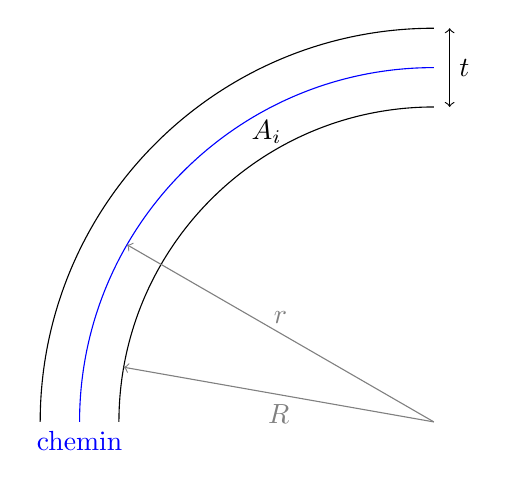
\begin{tikzpicture}[scale=2]

\def\R{2}
\def\r{2.25}
\def\A{2.5}

\draw[blue] (0,\r) arc (90:180:\r) node[below] {chemin};
\draw (0,\R) arc (90:180:\R);
\draw (0,\A) arc (90:180:\A);

\draw[->, gray] (0,0)--(150:\r) node[midway,above] {$r$};
\draw[->, gray] (0,0)--(170:\R) node[midway,below] {$R$};

\draw[<->] (0.1,\R)--(0.1,\A) node[right, midway] {$t$};

\node at (120:2.125) {$A_i$};

\end{tikzpicture}

\end{document}